\section{Mutable types}
\subsection{Lists}

\begin{frame}[fragile]
    \frametitle{List: definition}
    A list is an \emph{ordered} sequence of elements, which are \emph{not necessarily of the same type}. Each element of the list is assigned a unique \emph{index}, which is the element's position within the list.
   
        \begin{center}
    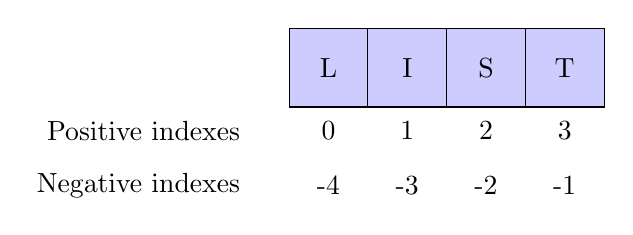
\begin{tikzpicture}
        \filldraw[step=1.0,black, thin, fill=blue!20] (0., 0. ) grid (4, 1) rectangle(0, 0);
        \draw (0.5, 0.5 ) node {L};
        \draw (1.5, 0.5 ) node {I};
        \draw (2.5, 0.5 ) node {S};
        \draw (3.5, 0.5 ) node {T};
        
        \def\wpos{-0.3}
        \def\wneg{-1}
        \def\lab{-0.5}

        \draw (0.5, \wpos ) node {0};
        \draw (1.5, \wpos ) node {1};
        \draw (2.5, \wpos ) node {2};
        \draw (3.5, \wpos ) node {3};
        \draw (\lab, \wpos ) node [anchor=east, align=right]{Positive indexes};
        
        \draw (0.5, \wneg ) node {-4};
        \draw (1.5, \wneg ) node {-3};
        \draw (2.5, \wneg ) node {-2};
        \draw (3.5, \wneg ) node {-1};
        \draw (\lab, \wneg ) node [anchor=east, align=right]{Negative indexes};
    \end{tikzpicture}
    \end{center}



    \begin{block}{Note}
        The \verb+sys.argv+ statements that was seen before returns the arguments as a list of strings
    \end{block}

\end{frame}

%\begin{frame}[fragile]
%\frametitle{List manipulation}
%\begin{lstlisting}
%x = [1] # initialisation
%x.append([1, 2, 3, 4]) # add list in list [1, [1, 2, 3, 4]]
%x.append('String') # add str in list [1, [1, 2, 3, 4], 'String']
%len(x) # 3
%
%x = [1]
%x.extend([1, 2, 3, 4]) # add list elmt. in list [1, 1, 2, 3, 4]
%x.extend('String')  # add list elmt. in list 
%#[1, 1, 2, 3, 4, 'S', 't', 'r', 'i', 'n', 'g']
%# strings are considered as a list of characters!
%len(x) # 11
%\end{lstlisting}
%\vspace{-0.8em}
%
%\begin{alertblock}{Warning!}
%No algebraic operations with list!
%\begin{lstlisting}
%x = [0, 1, 2]; y = [3, 4, 5]
%x + y # [0, 1, 2, 3, 4, 5] concatenation
%2*x # [0, 1, 2, 0, 1, 2]  concatenation
%\end{lstlisting}
%\end{alertblock}
%\end{frame}
%
%\begin{frame}[fragile]
%\frametitle{List manipulation}
%\begin{lstlisting}
%# removing list element
%x = range(15, 20) # [15, 16, 17, 18, 19]
%x.pop(2) # 2 = index of the elmt. to remove
%x # [15, 16, 18, 19]
%x.remove(16)  # Remove the first element matching 16 
%x # [15, 18, 19]
%\end{lstlisting}
%\begin{alertblock}{Caution when copying a list!}
%\begin{lstlisting}
%x = [1, 2, 3, 4, 5, 6, 7, 8, 9, 10]
%y = x
%x[4] = 30
%print y #[ 1  2  3  4 30  6  7  8  9 10]
%
%x = [1, 2, 3, 4, 5, 6, 7, 8, 9, 10]
%y = []
%y[:] = x
%x[4] = 30 
%print y #[ 1  2  3  4  5  6  7  8  9 10]
%\end{lstlisting}
%\end{alertblock}
%\end{frame}
%
%\begin{frame}[fragile]
%\frametitle{List manipulation}
%\begin{lstlisting}
%x = [5, 6, 15, 7, 2, 15]
%x.count(15)  # count occurrences of 15: 2
%
%x.reverse()  # reverse loop (in place!)
%x   # [15, 2, 7, 15, 6, 5]
%
%x.sort()  # sort elements (in place)
%x   # [2, 5, 6, 7, 15, 15]
%
%is7 = (7 in x)  # checks if 7 in the list
%is7  # True
%
%ind7 = x.index(7)  # finds index of 7 element
%ind7  # 3
%ind1000 = x.index(1000)  # error because 1000 not in list
%\end{lstlisting}
%
%\begin{alertblock}{Bad syntax!}
%\begin{lstlisting}
%x = x.reverse()
%x  # None
%\end{lstlisting}
%\end{alertblock}
%\end{frame}
%
%\begin{frame}[fragile]
%\frametitle{List indexing}
%Different from Matlab and R (can be confusing)
%\begin{lstlisting}
%list = [1, 2, 3, 4, 5, 6, 7, 8, 9, 10]
%print list[0] # 1, equivalent to list(1)
%print list[2:5] # [3,4,5] equivalent to list(3:5)
%print list[-1] # 10 equivalent to list(end)
%print list[-5:-3] # [6,7] equivalent to list(end-4:end-3)
%print list[6:] # [7, 8, 9, 10] eq. to list(7:end) 
%print list[:3] # [1,2,3] eq. to list(1:3)
%print list[2:-2:2] # [3, 5, 7] eq. to list(3:2:end-2)
%print list[::4] # [1, 5, 9] eq. to list(1:4:end)
%\end{lstlisting}
%\end{frame}
